\newcommand{\svcourse}{CST Part IA: Introduction to Probability}
\newcommand{\svnumber}{1}
\newcommand{\svvenue}{Churchill, Room TBD}
\newcommand{\svdate}{2022-05-14}
\newcommand{\svtime}{11:00}
\newcommand{\svuploadkey}{PO5ogKIM8KQA22FZS8IAf8gxA8XKi19jxIBVHIfFZ+3GCBXuNUXS9lVN6bNYjxM/}

\newcommand{\svrname}{Mr Matthew Ireland}
\newcommand{\jkfside}{twoside}
\newcommand{\jkfhanded}{right}

\newcommand{\studentname}{Harry Langford}
\newcommand{\studentemail}{hjel2@cam.ac.uk}


\documentclass[10pt,\jkfside,a4paper]{article}

\usepackage{mathtools}
\usepackage{tikz}
\usetikzlibrary{positioning}

% DO NOT add \usepackage commands here.  Place any custom commands
% into your SV work files.  Anything in the template directory is
% likely to be overwritten!

\usepackage{fancyhdr}

\usepackage{lastpage}       % ``n of m'' page numbering
\usepackage{lscape}         % Makes landscape easier

\usepackage{verbatim}       % Verbatim blocks
\usepackage{epsfig}         % Embed encapsulated postscript
\usepackage{array}          % Array environment
\usepackage[nolinks]{qrcode}         % QR codes
\usepackage{enumitem}       % Required by Tom Johnson's exam question header

\usepackage{hhline}         % Horizontal lines in tables
\usepackage{siunitx}        % Correct spacing of units
\usepackage{amsmath}        % American Mathematical Society
\usepackage{amssymb}        % Maths symbols
\usepackage{amsthm}         % Theorems

\usepackage{ifthen}         % Conditional processing in tex

\usepackage[top=3cm,
            bottom=3cm,
            inner=2cm,
            outer=5cm]{geometry}

% PDF metadata + URL formatting
\usepackage[
            pdfauthor={\studentname},
            pdftitle={\svcourse, SV \svnumber},
            pdfsubject={},
            pdfkeywords={9d2547b00aba40b58fa0378774f72ee6},
            pdfproducer={},
            pdfcreator={},
            hidelinks]{hyperref}

\renewcommand{\headrulewidth}{0.4pt}
\renewcommand{\footrulewidth}{0.4pt}
\fancyheadoffset[LO,LE,RO,RE]{0pt}
\fancyfootoffset[LO,LE,RO,RE]{0pt}
\pagestyle{fancy}
\fancyhead{}
\fancyhead[LO,RE]{{\bfseries \studentname}\\\studentemail}
\fancyhead[RO,LE]{{\bfseries \svcourse, SV~\svnumber}\\\svdate\ \svtime, \svvenue}
\fancyfoot{}
\fancyfoot[LO,RE]{For: \svrname}
\fancyfoot[RO,LE]{\today\hspace{1cm}\thepage\ / \pageref{LastPage}}
\fancyfoot[C]{\qrcode[height=0.8cm]{\svuploadkey}}
\setlength{\headheight}{22.55pt}

\ifthenelse{\equal{\jkfside}{oneside}}{

 \ifthenelse{\equal{\jkfhanded}{left}}{
  % 1. Left-handed marker, one-sided printing or e-marking, use oneside and...
  \evensidemargin=\oddsidemargin
  \oddsidemargin=73pt
  \setlength{\marginparwidth}{111pt}
  \setlength{\marginparsep}{-\marginparsep}
  \addtolength{\marginparsep}{-\textwidth}
  \addtolength{\marginparsep}{-\marginparwidth}
 }{
  % 2. Right-handed marker, one-sided printing or e-marking, use oneside.
  \setlength{\marginparwidth}{111pt}
 }

}{
 % 3. Alternating margins, two-sided printing, use twoside.
}

\setlength{\parindent}{0em}
\addtolength{\parskip}{1ex}

% Exam question headings, labels and sensible layout (courtesy of Tom Johnson)
\setlist{parsep=\parskip, listparindent=\parindent}
\newcommand{\examhead}[3]{\section{#1 Paper #2 Question #3}}
\newenvironment{examquestion}[3]{
    \examhead{#1}{#2}{#3}\setlist[enumerate, 1]{label=(\alph*)}\setlist[enumerate, 2]{label=(\roman*)}
    \marginpar{\qrcode{https://www.cl.cam.ac.uk/teaching/exams/pastpapers/y#1p#2q#3.pdf}}
    \marginpar{\footnotesize \url{https://www.cl.cam.ac.uk/teaching/exams/pastpapers/y#1p#2q#3.pdf}}
}{}



\begin{document}

\section{Notes Page 71}

\subsection*{Exercise 18}
What are the free variables of the following? Draw their
abstract syntax trees up to alpha equivalence.

\begin{enumerate}

\item $\text{fv}(x + ((\textbf{fn} \ y:\text{int} \Rightarrow z) 2)) = \{x, z\}$

\begin{center}
\begin{tikzpicture}
\node (root) {$\boldsymbol{\cdot} + \boldsymbol{\cdot}$};
\node (xleft) [below left = of root] {$\bullet$};
\path (xleft) edge (root);
\node (apply) [below right = of root] {@};
\path (apply) edge (root);
\node (funright) [below left = of apply] {$\textbf{fn} \ \boldsymbol{\cdot}:\text{int} \Rightarrow$};
\path (funright) edge (apply);
\node (zfun) [below = of funright] {$\bullet$};
\path [-stealth] (zfun) edge [bend right] (funright);
\path (zfun) edge (funright);
\node (two) [below right = of apply] {2};
\path (two) edge (apply);
\end{tikzpicture}
\end{center}

\item fv$(x + (\textbf{fn} \ y:\text{int} \Rightarrow z)) = \{x, z\}$

\begin{center}
\begin{tikzpicture}
\node (root) {$\boldsymbol{\cdot} + \boldsymbol{\cdot}$};
\node (xleft) [below left = of root] {$\bullet$};
\path (xleft) edge (root);
\node (funright) [below right= of root] {$\textbf{fn} \
\boldsymbol{\cdot}:\text{int} \Rightarrow$};
\path (funright) edge (root);
\node (zfun) [below = of funright] {$\bullet$};
\path [-stealth] (zfun) edge [bend right] (funright);
\path (zfun) edge (funright);
\end{tikzpicture}
\end{center}

\item fv$(\textbf{fn} \ y:\text{int} \Rightarrow \textbf{fn} \ y:\text{int} \Rightarrow
\textbf{fn} \ y:\text{int} \Rightarrow y) = \emptyset$

\begin{center}
\begin{tikzpicture}
\node (firstfun) {$\textbf{fn} \ \boldsymbol{\cdot}:\text{int} \Rightarrow$};
\node (secondfun) [below = of firstfun] {$\textbf{fn} \ \boldsymbol{\cdot}:\text{int}
\Rightarrow$};
\path (secondfun) edge (firstfun);
\node (thirdfun) [below = of secondfun] {$\textbf{fn} \ \boldsymbol{\cdot}:\text{int}
\Rightarrow$};
\path (thirdfun) edge (secondfun);
\node (y) [below = of thirdfun] {$\bullet$};
\path (y) edge (thirdfun);
\path [-stealth] (y) edge [bend right] (thirdfun);
\end{tikzpicture}
\end{center}

\item fv$(!\ell_0) = \emptyset$

\begin{center}
\begin{tikzpicture}
\node (deref) {$!\ell_0$};
\end{tikzpicture}
\end{center}

\item fv$(\textbf{while} \ !\ell_0 \geq y \ \textbf{do} \ \ell_0 \coloneqq
x) = \{x, y\}$

\begin{center}
\begin{tikzpicture}
\node (while) {$\textbf{while} \ \boldsymbol{\cdot} \ \text{do} \
\boldsymbol{\cdot}$};
\node (geq) [below left = of while] {$\boldsymbol{\cdot} \geq \boldsymbol{\cdot}$};
\path (geq) edge (while);
\node (deref) [below left = of geq] {$!\ell_0$};
\path (deref) edge (geq);
\node (geqx) [below right = of geq] {$\bullet$};
\path (geqx) edge (geq);
\node (assign) [below right = of while] {$\ell_0\coloneqq \cdot$};
\path (assign) edge (while);
\node (assignx) [below = of assign] {$\bullet$};
\path (assignx) edge (assign);
\end{tikzpicture}
\end{center}

\end{enumerate}

\subsection*{Exercise 19}
What are the results of the following substitutions?

\begin{enumerate}

\item $\{\textbf{fn} \ x: \text{int} \Rightarrow y / z\}\textbf{fn} \
y:\text{int} \Rightarrow z \ y$

\[
\textbf{fn} \ z:\text{int} \Rightarrow (\textbf{fn} \ x: \text{int}
\Rightarrow y) \ z
\]

\item $\{\textbf{fn} \ x: \text{int} \Rightarrow x / x\}\textbf{fn} \
y:\text{int} \Rightarrow x \ y$

\[
\textbf{fn} \ y:\text{int} \Rightarrow (\textbf{fn} \ x: \text{int}
\Rightarrow x) \ y
\]

\item $\{\textbf{fn} \ x:\text{int} \Rightarrow x / x\}\textbf{fn} \
x:\text{int} \ x \ x$

\[
\textbf{fn} \ x:\text{int} \ x \ x
\]

\end{enumerate}

\subsection*{Exercise 21}

Give a grammar for types, and typing rules for functions and application
that allow only first order functions and prohibit partial applications.

Types:
\begin{align*}
A &\Coloneqq \ \text{int} \ | \ \text{bool} \ | \ \text{unit} \\
T &\Coloneqq \ A \ | \ A \rightarrow A \\
T_{loc} &\Coloneqq \text{intref} \\
\end{align*}

Typing rules:
\begin{gather*}
\dfrac{}{\Gamma \vdash n: \text{int}} \\\\
\dfrac{}{\Gamma \vdash b: \text{bool}} \\\\
\dfrac{}{\Gamma \vdash \textbf{skip}: \text{unit}} \\\\
\dfrac{
\Gamma \vdash e: A'
}{
\Gamma \vdash \textbf{fn} \ x:A \Rightarrow e: A \rightarrow A'
}\\\\
\dfrac{
\Gamma \vdash \textbf{fn} \ x:A \Rightarrow e: A \rightarrow A'
\ \ \
\Gamma \vdash e': A
}{
\Gamma \vdash (\textbf{fn} \ x:A \Rightarrow e)e': A'
}
\end{gather*}

\subsection*{Exercise 24}

Prove Theorem 19 (Type Preservation) for recursive functions

Continue the proof from last supervision with $\Phi(e, s, e', s', T)$ defined
the same:

\[
\Phi(e, s, e', s', T) \triangleq \left(\Gamma \vdash e: T \wedge \langle e, s
\rangle \to \langle e', s' \rangle\right) \Longrightarrow \Gamma \vdash e': T
\]

\begin{itemize}

\item [\textbf{Case}] (letrecfn) Recall the evaluation rule:
\begin{gather*}
\langle \textbf{let val rec} \ x : T_1 \to T_2 = (\textbf{fn} \ y: T_1
\Rightarrow e_1) \ \textbf{in} \ e_2 \ \textbf{end}, s\rangle \\
\to \\
\langle \{(\textbf{fn} \ y: T_1 \Rightarrow \textbf{let val rec} \ x : T_1 \to T_2 = (\textbf{fn} \ y: T_1
\Rightarrow e_1) \ \textbf{in} \ e_1 \ \textbf{end})/x\}e_2, s \rangle
\end{gather*}

Recall also the typing rule (let rec fn):
\[
\dfrac{
\Gamma, x: T_1 \to T_2, y: T_1 \vdash e_1: T_2 \ \ \ \Gamma, x: T_1 \to T_2
\vdash e_2: T
}{
\Gamma \vdash \textbf{let val rec} \ x : T_1 \to T_2 = (\textbf{fn} \ y: T_1
\Rightarrow e_1) \ \textbf{in} \ e_2 \ \textbf{end}: T
}
\]

There is no other typing rule with a conclusion of the form \textbf{let val
rec} \ldots \ \textbf{end}. Therefore (let rec fn) must have been the last
typing rule used and so we can infer the premises of the rule $\Gamma, x:
T_1 \to T_2, y: T_1 \vdash e_1 : T_2$ and $\Gamma, x : T_1 \to T_2 \vdash
e_2 : T$.

Since the reduced expression is $e_2$ with an expression of type $T_1 \to
T_2$ for $x$ and the premise states that under $\Gamma$ and the assumption
that $x: T_1 \to T_2$, $e_2 : T$; we can conclude that $\{\dots/x\}e_2$ has
type $T$.

Since the type of the reduced expression is the same as the type of the
original expression, we can conclude $\Phi(e, s, e', s', T)$ as required.

\end{itemize}

\begin{examquestion}{2015}{6}{10}

\begin{enumerate}[label=(\alph*)]

\setcounter{enumi}{1}

\item Define a small-step right-to-left call-by-value operational semantics
for this syntax.

\begin{align*}
(\text{reduce}) \ \ \ &
\dfrac{
\langle e_1 \rangle \stackrel{L}{\to} \langle e_1' \rangle
}{
\langle e_1 \ e_2 \rangle \stackrel{L}{\to} \langle e_1' \ e_2 \rangle
}
&
(\text{arg}) \ \ \ &
\dfrac{
\langle e_2 \rangle \stackrel{L}{\to} \langle e_2' \rangle
}{
\langle (\textbf{fn} \ x \Rightarrow e_1) \ e_2 \rangle \stackrel{L}{\to} \langle (\textbf{fn}
\ x \to e_1) \ e_2' \rangle
} \\
(\text{printarg}) \ \ \ &
\dfrac{
\langle e \rangle \stackrel{L}{\to} \langle e' \rangle
}{
\langle \mathbf{print} \ e \rangle \stackrel{L}{\to} \langle \mathbf{print} \ e' \rangle
}
&
(\text{call}) \ \ \ &
\dfrac{
}{
\langle (\textbf{fn} \ x \Rightarrow e) \ v \rangle \stackrel{\tau}{\to}
\langle \{v/x\}e \rangle
} \\
(\text{print}) \ \ \ &
\dfrac{
}{
\langle \mathbf{print} \ n \rangle \stackrel{n}{\to} \langle \mathbf{skip}
\rangle
}
\end{align*}

\setcounter{enumi}{3}

\item We are normally interested in closed programs (with no free variables).
Prove with respect to your call-by-value semantics of part (\textit{b}) that
if \textit{e} is closed and $e \stackrel{L}{\longrightarrow} e'$ then $e'$
is closed. You can omit the cases for \textbf{print}.

An expression $e$ is closed if and only if $\mathbf{fv}(e) = \emptyset$. 
Therefore we must prove for all closed expressions $e$, the property $\Phi$:

\[
\Phi(e) \triangleq \forall e'. \left( \mathbf{fv} (e) = \emptyset \wedge
\langle e \rangle \stackrel{L}{\to} \langle e' \rangle \right)
\Longrightarrow (\mathbf{fv}(e') = \emptyset)
\]

This can be performed by structural induction on the evaluation rules using the
induction hypothesis $\Phi(e)$ for all subexpressions $e$.

\begin{enumerate}[label=(\textbf{Case})]

\item (reduce) Recall the rule (reduce):
\[
\dfrac{
\langle e_1 \rangle \stackrel{L}{\to} \langle e_1' \rangle
}{
\langle e_1 \ e_2 \rangle \stackrel{L}{\to} \langle e_1' \ e_2 \rangle
}
\]

By assumption $\mathbf{fv}(e) = \emptyset$. Using this and
the formula for the free variables of $e_1 \ e_2$ gives:
\[
\begin{split}
\mathbf{fv}(e_1 \ e_2) &= \mathbf{fv}(e_1)\cup\mathbf{fv}(e_2)
\wedge \mathbf{fv}(e_1 \ e_2) = \emptyset \Longrightarrow \\
\mathbf{fv}(e_1) &= \mathbf{fv}(e_2) = \emptyset \\
\end{split}
\]

\[
\begin{split}
&\Phi(e_1) \wedge \mathbf{fv}(e_1) = \emptyset \wedge \langle e_1\rangle
\stackrel{L}{\to}\langle e_1' \rangle \Longrightarrow \\
&\mathbf{fv}(e_1') = \emptyset \Longrightarrow \\
&\mathbf{fv}(e_1' \ e_2) = \emptyset \Longrightarrow \\
&\Phi(e_1 \ e_2)\\
\end{split}
\]

\item (arg) Recall the rule:
\[
\dfrac{
\langle e_2 \rangle \stackrel{L}{\to} \langle e_2' \rangle
}{
\langle (\textbf{fn} \ x \Rightarrow e_1) \ e_2 \rangle \stackrel{L}{\to} \langle (\textbf{fn}
\ x \to e_1) \ e_2' \rangle
}
\]

By assumption, $\mathbf{fv}((\textbf{fn} \ x \Rightarrow e_1) \ e_2) =
\emptyset$.

\[
\begin{split}
&\mathbf{fv}((\textbf{fn} \ x \Rightarrow e_1) \ e_2) = \emptyset
\Longrightarrow \\
&\mathbf{fv}(\textbf{fn} \ x \Rightarrow e_1) = \emptyset \wedge \mathbf{fv}
(e_2) = \emptyset \\
\end{split}
\]

Since $e_2$ is a subexpression of $e$, the induction hypothesis $\Phi(e_2)$
holds.

\[
\begin{split}
&\Phi(e_2) \wedge \mathbf{fv}(e_2) = \emptyset \wedge \langle e_2 \rangle
\stackrel{L}{\to} \langle e_2' \rangle \Longrightarrow \\
&\mathbf{fv}(e_2') = \emptyset \\
\end{split}
\]

\[
\begin{split}
&\mathbf{fv}(\textbf{fn} \ x \Rightarrow e_1) = \emptyset \wedge \mathbf{fv}
(e_2') = \emptyset  \Longrightarrow \\
&\mathbf{fv}((\textbf{fn} \ x \Rightarrow e_1) \ e_2') = \emptyset
\Longrightarrow \\
&\Phi((\textbf{fn} \ x \Rightarrow e_1) \ e_2') \\
\end{split}
\]

\item (call) Recall the rule:

\[
\dfrac{
}{
\langle (\textbf{fn} \ x \Rightarrow e) \ v \rangle \stackrel{\tau}{\to}
\langle \{v/x\}e \rangle
}
\]

By induction hypothesis:
\[
\Phi(\mathbf{fn} \ x \Rightarrow e)
\Longrightarrow \mathbf{fv}(x \Rightarrow e) = \emptyset
\]

\[
\begin{split}
&\mathbf{fv}(\mathbf{fn} \ x \Rightarrow e) = \mathbf{fv}(e) - \{x\} \wedge
\mathbf{fv}(x \Rightarrow e) = \emptyset \Longrightarrow \\
&\mathbf{fv}(e) \subseteq \{x\} \Longrightarrow \\
&\mathbf{fv}(\{v/x\}e) \subseteq \{x\} - \{x\} \Longrightarrow \\
&\mathbf{fv}(\{v/x\}e) = \emptyset \Longrightarrow \\
&\Phi((\textbf{fn} \ x \Rightarrow e) \ v) \\
\end{split}
\]

\end{enumerate}

Since all cases have been proved, we can conclude that $\forall e. \Phi(e)$.
As required.

\end{enumerate}

\end{examquestion}

\begin{examquestion}{2008}{6}{11}

Below is the syntax and type system for a simple functional language.

Integers $n \in \mathbb{Z} = \{\dots, -1, 0, 1, \dots\}$\\
Variables $x \in \mathbb{X} = \{x, y, z\}$\\
Types $T \Coloneqq \text{int} \ | \ T \to T$ \\
Type environments $\Gamma$, finite partial functions from variables to types.\\
Expressions $e \Coloneqq n \ | \ x \ | \ \textbf{fn} \ x:T \Rightarrow e \ |
\ e_1 \ e_2 $

\begin{align*}
(\text{int}) \ \ \ & \Gamma \vdash n: \text{int} \ \text{for} \ n \in
\mathbb{Z}
&
(\text{var}) \ \ \ & \Gamma \vdash x: T \ \text{if} \ \Gamma(x) = T \\
(\text{fn}) \ \ \ & \dfrac{\Gamma, x:T \vdash e: T'}{\Gamma \vdash \textbf{fn} \
x: T \Rightarrow e : T \to T'}
&
(\text{app}) \ \ \ &
\dfrac{\Gamma \vdash e_1: T \to T' \ \ \ \Gamma \vdash e_2: T}{\Gamma \vdash
 e_1 \ e_2: T'}
\end{align*}

\begin{enumerate}[label=(\alph*)]

\item Give a call-by-value operational semantics for this language, defining
a judgement $e \to e'$ (the language does not have store operations so you
can take configurations to be just expressions).
\begin{align*}
(\text{call1}) &
\dfrac{\langle e \rangle \to \langle e' \rangle }
{\langle (\textbf{fn} \ x \Rightarrow e'') \ e \rangle
\to
\langle (\textbf{fn} \ x \Rightarrow e'') \ e' \rangle
}
\\\\
(\text{call2}) &
\dfrac{}{
\langle (\textbf{fn} \ x \Rightarrow e) \ n \rangle
\to
\langle \{n/x\}e \rangle
} \\
\end{align*}

\item Give an example of a stuck configuration.
\[
\langle x \rangle
\]

\item Prove the substitution lemma stated below:
\[
\text{If} \ \Gamma , x: T \vdash e': T' \ \text{and} \ \Gamma \vdash e : T
\ \text{with} \ x \notin \text{dom}(\Gamma) \ \text{then} \ \Gamma \vdash
\{e/x\}e': T'
\]

Define $\Phi(e, e', x)$ as follows:
\[
\Phi(e, e', x) \triangleq
\forall \Gamma, x, T, T'.
\left(\Gamma, x: T \vdash e': T' \wedge \Gamma \vdash e:
T \wedge x \notin \text{dom}(\Gamma)\right) \Longrightarrow \Gamma \vdash
 \{e/x\}e': T'
\]

This can be proved by structural induction over the typing rules. By
assumption, $\Gamma, x:T \vdash e': T'$. Therefore, $e'$ must be well typed
and must have been derived by the typing rules. The induction hypothesis is
$\Phi(e, e'', x)$ for all subexpressions $e''$ of $e'$.

\begin{itemize}[label=\textbf{Case}]

\item (int) Recall the typing rule:

\[
\dfrac{n \in \mathbb{Z}}{\Gamma \vdash n: \text{int}}
\]

If the last typing rule applied was (int), then $e'$ must be of the form
$n$. $\{e/x\}n = n$.
\[
\begin{split}
&\Gamma \vdash n : T \wedge \{e/x\}n = n \Longrightarrow \\
&\Gamma \vdash \{e/x\}n : T \ \text{as required}
\end{split}
\]

\item (var) Recall the typing rule:
\[
\dfrac{
\Gamma(y) = T
}{
\Gamma \vdash y: T
}
\]

\begin{enumerate}[label=\textbf{case}]

\item $x \neq y$

If $x \neq y$ then $\{e/x\}y = y$
\[
\begin{split}
&\Gamma \vdash y: T \wedge \{e/x\}y = y \Longrightarrow \\
&\Gamma \vdash \{e/x\}y : T \ \text{as required} \\
\end{split}
\]

\item $x = y$

If $x = y$ then $\{e/x\}y = e$
\[
\begin{split}
&\Gamma \vdash x: T \wedge \{e/x\}y = e \wedge \Gamma \vdash e: T
\Longrightarrow \\
&\Gamma \vdash \{e/x\}y: T \ \text{as required}
\end{split}
\]

\end{enumerate}

\item (fn) Recall the typing rule:

\[
\dfrac{
\Gamma, y:T \vdash e'': T'
}{
\Gamma \vdash \textbf{fn} \ y: T \Rightarrow e'' : T \to T'
}
\]

By the induction hypothesis $\Phi(e, e'', x)$ and the premise of the rule (fn):
\[
\begin{split}
&\Gamma, y: T \vdash e'': T' \wedge \Phi(e, e'', x) \Longrightarrow \\
&\Gamma, y: T \vdash \{e/x\}e'': T'
\end{split}
\]

Using the rule (fn):

\[
\dfrac{
\Gamma, y:T \vdash \{e/x\}e'': T'
}{
\Gamma \vdash \textbf{fn} \ y: T \Rightarrow \{e/x\}e'' : T \to T'
}
\]

Since the premise of this is implied by the induction hypothesis, we can
assume the conclusion.

Since $y$ binds, $x$ cannot occur in $y$. The required result is obtained.
\[
\mathbf{fn} \ y \Rightarrow\{e/x\}e'' = \{e/x\}(\mathbf{fn} \ y \Rightarrow e'')
\]

\item (app) Recall the rule:

\[
\dfrac{
\Gamma \vdash e_1: T \to T' \ \ \ \Gamma \vdash e_2: T
}{
\Gamma \vdash e_1 \ e_2: T'
}
\]

Using the induction hypothesis $\Phi(e, e_1, x)$ and $\Phi(e, e_2, x)$, we
can infer $\Gamma \vdash \{e/x\}e_1: T\to T'$ and $\Gamma \vdash \{e/x\}e_2:
 T$. Substituting this into the rule above gives:

\[
\dfrac{
\Gamma \vdash \{e/x\}e_1: T \to T' \ \ \ \Gamma \vdash \{e/x\}e_2: T
}{
\Gamma \vdash \{e/x\}e_1 \ \{e/x\}e_2: T'
}
\]

The conclusion is the same as substituting $e$ for $x$ in the whole
expression. Substituting this equality into the evaluation rule gives the
required result:

\[
\dfrac{
\Gamma \vdash \{e/x\}e_1: T \to T' \ \ \ \Gamma \vdash \{e/x\}e_2: T
}{
\Gamma \vdash \{e/x\}(e_1 \ e_2): T'
}
\]

\end{itemize}

Therefore, the if the substitution principle holds for all subexpressions of
$e$ then it also holds for $e$. Since the substitution principle holds for
all nullary expressions it must therefore hold for all expressions.

\item State and prove type preservation, using the substitution lemma.

Type preservation $\Phi$ for an expression $e$ is defined as:

\[
\Phi(e) \triangleq \forall \Gamma, T, e'. \Gamma \vdash e: T \wedge \langle e
\rangle \to \langle e' \rangle \Rightarrow \Gamma \vdash e': T
\]

To prove this, we can assume the LHS of the implication and prove the RHS .
We assume that $\Gamma \vdash e: T$. So $e$ is well-typed and so must
conform to the typing rules. We can perform structural induction on the last
typing rule used.

\begin{enumerate}[label=\textbf{Case}]

\item (int)

If the last typing rule used was (int), then $\exists n \in \mathbb{Z}. e =
n$. Therefore there is no reduction from $e$. Hence the LHS of the
implication does not hold and type preservation trivially holds in this case.

\item (var)

If the last typing rule used was (var), then $e$ must be a variable. Since
there are no evaluation rules which can have a varaible in the premise, $e$
can therefore not reduce and so type preservation trivially holds in this case.

\item (fn)

If the last typing rule used was (fn) then $e$ must be of the form
$\mathbf{fn} \ x \to e_1$. There is no evaluation rule with an expression of
this form as the premise and therefore type preservation holds trivially as
$e$ cannot reduce.

\item (app)

If the last typing rule used was (app) then $e$ must be of the form $e_1 \
e_2$. Perform a case split on $e_2$:

\begin{enumerate}[label=\textbf{case}]

\item $e_2 \in \mathbb{Z}$

In this case, we can apply the rule (call2):
\[
\dfrac{}{
\langle (\mathbf{fn} \ x \Rightarrow e) \ n \rangle \to \langle \{n/x\}e \rangle
}
\]

By use of the substitution principle:
\[
\Gamma, x: T \vdash e' : T' \wedge \Gamma e: T \wedge x \notin \text{dom}
(\Gamma) \Longrightarrow \Gamma \vdash \{e/x\}e': T'
\]

Therefore the type of $\{n/x\}e$ must be $T$. Since the function took $n$ as
an argument, it must have type $\text{int} \to T$. Therefore we can apply
the typing rule (app) and derive that the type of $e \ n$ must be $T$.
Therefore the type of the expression was preserved in this reduction and so
type preservation holds in this case.

\item $e_2 \notin \mathbb{Z}$

By assumption, $\Gamma \vdash e_2 : T$:

\[
\begin{split}
&\Gamma \vdash e_2 : T \wedge e_2 \notin \mathbb{Z} \Longrightarrow \\
&\exists e_2'. \langle e_2 \rangle \to \langle e_2' \rangle
\end{split}
\]

By induction hypothesis, type preservation holds on reductions for $e_2$.
Therefore the type of $e_2'$ must be the same as the type of $e_2$ -- let
this type be $T$. By use of the rule (app):

\begin{align*}
&
\dfrac{
\Gamma \vdash e_2: T \to T' \ \ \ \Gamma \vdash e_2: T
}{
\Gamma \vdash e_1 \ e_2: T'
}
&
\dfrac{
\Gamma \vdash e_2: T \to T' \ \ \ \Gamma \vdash e_2': T
}{
\Gamma \vdash e_1 \ e_2': T'
}
\end{align*}

\end{enumerate}

\end{enumerate}

\end{enumerate}

\end{examquestion}

\section{Exercises Page 85}

\subsection*{Exercise 18}

Labelled variant types are a generalisation of sum types, just as
records are a generalisation of products. Design abstract syntax, type rules
and evaluation rules for labelled variants, analagously to the way in which
records generalise products.

Abstract Syntax:
\[
\begin{split}
lab &\in \mathbb{LAB} = \{p, q, \dots\} \\
T &\Coloneqq \dots \ | \ T_1 + T_2 + \dots + T_n \\
e &\Coloneqq \dots \ | \ lab_1[e:T_1] \ | \ lab_2[e:T_2] \ | \ \dots \ | \
lab_n(e: T_n)
\end{split}
\]

Typing Rules:
\begin{gather*}
(\text{Variant}) \ \ \
\dfrac{
\Gamma \vdash e: T_i
}{
\Gamma \vdash lab_i(e): T_1 + T_2 + \dots + T_n
} \\\\
(\text{Case}) \ \ \
\dfrac{
\begin{matrix}
\Gamma \vdash e: T_1 + T_2 + \dots + T_n \\
\Gamma \vdash x_i: T_i \vdash e_i: T \\
\end{matrix}
}{
\Gamma \vdash (\textbf{case} \ e \ \text{of} \ lab_1(x_1: T_1) \Rightarrow
e_1: T \ | \ \dots
\ | \ lab_n(x_n: T_n) \Rightarrow e_n: T):T
}
\end{gather*}

Evaluation Rules:
\begin{gather*}
(\text{lab}) \ \ \
\dfrac{
\langle e, s \rangle \to \langle e', s' \rangle
}{
\langle
lab_i(e: T_i), s
\rangle
\to
\langle
lab_i(e': T_i), s'
\rangle
}\\\\
(\text{case1}) \ \ \
\dfrac{
\langle e, s \rangle \to \langle e', s' \rangle
}{
\begin{matrix}
\langle \textbf{case} \ e \ \text{of} \ lab_1(x_1: T_1) \Rightarrow e_1 \ | \
\dots
\ | \ lab_n(x_n: T_n) \Rightarrow e_n, s \rangle\\
\to \\
\langle \textbf{case} \ e' \ \text{of} \ lab_1(x_1: T_1) \Rightarrow e_1 \ | \
\dots
\ | \ lab_n(x_n: T_n) \Rightarrow e_n, s' \rangle \\
\end{matrix}
}\\\\
(\text{casematch}) \ \ \
\dfrac{
}{
\begin{matrix}
\langle \textbf{case} \ lab_i \ v \ \text{of} \ lab_1(x_1: T_1) \Rightarrow
e_1 \ | \ \dots\ | \ lab_n(x_n: T_n) \Rightarrow e_n, s \rangle \\
\to \\
\langle \{v/x_i\}e_i, s\rangle
\end{matrix}
}
\end{gather*}

\section{Notes Page 92}

\subsection*{Exercise 32}

For each of the two bogus $T$ ref subtype rules on Slide 202, give an
example program that is typeable with that rule but gets stuck at runtime.

This program will pass typechecking but get stuck at runtime under the first
rule.

\[
\begin{split}
\langle&\\
&\ell \coloneqq \{p = 1\} \\
&\#q \ !\ell, \\
&\{\ell \mapsto \{p=0, q=0\}\}\\
&\rangle \\
\end{split}
\]

This program will pass typechecking but get stuck at runtime under the
second rule:

\[
\begin{split}
\langle & \\
&\#q \ !\ell, \\
&\{\ell\mapsto \{p=0\}\}\\
&\rangle \\
\end{split}
\]

\subsection*{Exercise 33}

What should the subtype rules for sums $T + T'$ be?

\begin{gather*}
(\text{sum1}) \ \ \ \dfrac{
T <\vcentcolon T''
}{
T + T' <\vcentcolon T'' + T'
}\\\\
(\text{sum2}) \ \ \ \dfrac{
T' <\vcentcolon T''
}{
T + T <\vcentcolon T + T''
}
\end{gather*}

\begin{examquestion}{2014}{6}{10}

Consider the language $L$ below, with call-by-value functions, ML-style
references and types $\mathbf{nat}_+$ and $\mathbf{real}_+$ of positive
natural and positive real numberes. $L$ includes a primitive test for
primality, $\mathbf{prime}(e)$ and a square root funciton, $\mathbf{sqrt}(e)
$; these are defined only for positive-natural and positive-real values
respectively.

\[
\begin{split}
T &\coloneqq \mathbf{bool} \ | \ \mathbf{nat}_+ \ | \ \mathbf{real}_+ \ | \ T
 \to T' \ | \ T \ \mathbf{ref} \\
e &\coloneqq x \ | \ n \ | \ r \ | \ \mathbf{fn} \ x : T \Rightarrow e \ | \ e
\ e'
\ | \ \mathbf{ref} \ e \ | \ !e \ | \ e \coloneqq e' \ | \ \mathbf{prime}(e) \
 | \ \mathbf{sqrt}(e)
\end{split}
\]

Here $x$ ranges over a set $X$ of variables and $n$ and $r$ range over
$\mathbb{N}_{> 0}$ and $\mathbb{R}_{>0}$ respectively. Let $\Gamma$ range
over finite partial functions from $X$ to types $T$.

\begin{enumerate}[label=(\alph*)]

\item Give typing rules defining $\Gamma \vdash  e : T$ for $\mathbf{prime}
(e)$ and $\mathbf{sqrt}(e)$.

\[
\begin{split}
(\text{prime}) \ \ \
\dfrac{
\Gamma \vdash e: \mathbf{nat}_+
}{
\Gamma \vdash \mathbf{prime}(e) : \mathbf{bool}
}\\\\
(\text{sqrt}) \ \ \
\dfrac{
\Gamma \vdash e: \mathbf{real}_+
}{
\Gamma \vdash \mathbf{sqrt}(e): \mathbf{real}_+
}
\end{split}
\]

There is an obvious runtime coercion from elements of $\mathbf{nat}_+$ to
elements of $\mathbf{real}_+$. To let programmers exploit that conveniently,
we would like to define a type system from $L$ that includes a subtype
relation $T_1 <\vcentcolon T_2$ with $\mathbf{nat}_+ <\vcentcolon \mathbf{real}_+$.
The type system should prevent all runtime errors.

\begin{enumerate}[label=(\roman*)]

\item Give the other rules defining $T_1 <\vcentcolon T_2$ and the subsumption rule to
use that relation in $\Gamma \vdash e: T$.

\begin{align*}
(\text{reflexivity}) \ \ \  &
\dfrac{}{T <\vcentcolon T}
&
(\text{transitivity}) \ \ \ &
\dfrac{T_1 <\vcentcolon T_2 \wedge T_2 <\vcentcolon T_3}{T_1 <\vcentcolon T_3}
\\\\
(\text{subsumption})\ \ \ &
\dfrac{
\Gamma \vdash e: T \ \ \ T <\vcentcolon T'
}{
\Gamma \vdash e: T'
}
&
(\text{function}) \ \ \ &
\dfrac{
T_1 <\vcentcolon T_1' \wedge T_2 <\vcentcolon T_2'
}{
(T_1' \to T_2) <\vcentcolon (T_1 \to T_2')
}
\end{align*}

\item Give the 6 (standard) typing rules defining $\Gamma \vdash e: T$ for
functions and references.

\begin{align*}
(\text{fn}) \ \ \ &
\dfrac{
\Gamma, x:T \vdash e: T'
}{
\Gamma \vdash \mathbf{fn} \ x: T \Rightarrow e: T \to T'
}
&
(\text{apply}) \ \ \ &
\dfrac{
\Gamma \vdash e_1: T \to T' \ \ \ \Gamma \vdash e_2: T
}{
\Gamma \vdash e_1 \ e_2: T'
}\\\\
(\text{ref}) \ \ \ &
\dfrac{
\Gamma \vdash e: T
}{
\Gamma \vdash \mathbf{ref} \ e: T \ \mathbf{ref}
}
&
(\text{assign}) \ \ \ &
\dfrac{
\Gamma \vdash e: T \ \mathbf{ref} \ \ \ \Gamma \vdash e': T
}{
\Gamma \vdash e \coloneqq e': T
}\\\\
(\text{deref}) \ \ \ &
\dfrac{
\Gamma \vdash e: T \ \mathbf{ref}
}{
\Gamma \vdash \ !e: T
}
&
(\text{loc}) \ \ \ &
\dfrac{
\Gamma(\ell) = T \ \mathbf{ref}
}{
\Gamma \vdash \ell: T \ \mathbf{ref}
}
\end{align*}

\item With reference to your subtype rule for function types, explain
covariance and contravariance of subtyping. Give examples in $L$ showing that
your rule is the only reasonable choice.

Functions have contravariant argument types and covariant return types. It
must be this way to ensure that every function takes a type with at least as
much information as it requires and returns types with at least as much
information as the context is expecting.

Consider the following example code which passes typechecking but gets stuck
at runtime when we have covariant argument types:
\begin{gather*}
\dfrac{
T_1 <\vcentcolon T_1' \wedge T_2 <\vcentcolon T_2'
}{
(T_1 \to T_2) <\vcentcolon (T_1' \to T_2')
}\\\\
\langle \mathbf{sqrt}((\mathbf{fn} \ x: \mathbf{real}_+ \to x) \ 0) \rangle
\longrightarrow^* \langle \mathbf{sqrt}(0) \rangle \not\to
\end{gather*}

Consider the following example which passes typechecking but get stuck at
runtime when we have contravariant
return types:
\begin{gather*}
\dfrac{
T_1 <\vcentcolon T_1' \wedge T_2 <\vcentcolon T_2'
}{
(T_1' \to T_2') <\vcentcolon (T_1 \to T_2)
}\\\\
\langle \mathbf{prime}((\mathbf{fn} \ x: \mathbf{nat}_+ \to x) \ 3.14)
\rangle \to \langle \mathbf{prime}(3.14) \rangle \not\to
\end{gather*}

\item Similarly, justify your rule for reference types.

There is no subtyping rule for reference types. If we have either covariant
or contravariant reference types, then we must disallow either reading or
writing to the reference to ensure type safety. This defeats the purpose of
references, rendering them useless.

Consider the following example which passes typechecking with covariant
references but gets stuck at runtime.
\begin{gather*}
\dfrac{
T <\vcentcolon T'
}{
T \ \mathbf{ref} <\vcentcolon T' \ \mathbf{ref}
}\\\\
\langle \mathbf{sqrt}(!(\mathbf{ref} \ 3)) \rangle \to \langle \mathbf{sqrt}
(3) \rangle \not\to
\end{gather*}

Consider the following example which passes typechecking with contravariant
references but gets stuck at runtime.

\begin{gather*}
\dfrac{
T <\vcentcolon T'
}{
T \ \mathbf{ref} <\vcentcolon T' \ \mathbf{ref}
}\\\\
\langle \mathbf{prime}(!(\mathbf{ref} \ 3.14)) \rangle
\to \langle \mathbf{prime}(3.14) \rangle \not\to
\end{gather*}

\end{enumerate}

\item To implement L, we want to translate it during typechecking to another
typed language $L'$ which makes that coercion explicit where requires, as a
new expression form $\mathbf{real\_of\_nat}(e)$ and which does not have
subtyping.

\begin{enumerate}[label=(\roman*)]

\item Give the $L'$ typing rule for $\mathbf{real\_of\_nat}(e)$ and indicate any
other changes required to your type rules for L.

\begin{align*}
(\text{real\_of\_nat}) \ \ \ &
\dfrac{
\Gamma \vdash e: \mathbf{nat}_+
}{
\Gamma \vdash \mathbf{real\_of\_nat}(e): \mathbf{real}_+
}\\
\end{align*}

We need to expand the set of expressions to include $\mathbf{real\_of\_nat}$.

\[
e \Coloneqq \dots \ | \ \mathbf{real\_of\_nat}
\]

\item Define an inductive relation $T <\vcentcolon T' \rightsquigarrow e$ for which
any $T <\vcentcolon T'$ constructs a coercion $e: T: T'$.

\[
(\text{reflexive}) \ \ \
\dfrac{
}{
T <: T \rightsquigarrow \mathbf{fn} \ x \Rightarrow x
}
\]

I spent a lot of time failing to understand what this question meant. After 2
days, I decided it was better to answer 95\% than 0\% and looked at the
first rule for (ii) (reflexivity) to figure out what it wanted. I hope that
was acceptable. The rest of (ii) and entirety of (iii) is mine.

\begin{align*}
(\text{real\_of\_nat}) \ \ \ &
\dfrac{
}{
\mathbf{nat}_+ <: \mathbf{real}_+ \rightsquigarrow
\mathbf{fn} \ x \Rightarrow \mathbf{real\_of\_nat}(x)
}\\\\
(\text{fn}) \ \ \ &
\dfrac{
T_1' <: T_1 \rightsquigarrow e_1 \ \ \
T_2 <: T_2' \rightsquigarrow e_2
}{
T_1 \to T_2 <: T_1' \to T_2' \rightsquigarrow \mathbf{fn} \ x \Rightarrow
(\mathbf{fn} \ y \Rightarrow e_2 \ y) \ (e_1 \ x)
}
\end{align*}

\item Define an inductive relation $\Gamma \vdash e \rightsquigarrow e': T $
where $e$ is an $L$ expression and $e'$ is an $L'$ expression which is like $e$
but with coercion introduced where needed, such that $\Gamma \vdash e: T$
iff $\exists e'. \Gamma \vdash e \rightsquigarrow e': T$. You should explain
but need not prove that, and you can omit the rules for references.

\begin{align*}
(\text{var})\ \ \ & \dfrac{}{x \rightsquigarrow x} &
(\text{nat})\ \ \ & \dfrac{}{n \rightsquigarrow n} &
(\text{real})\ \ \ & \dfrac{}{r \rightsquigarrow r}
\end{align*}
\[
(\text{real\_of\_nat})\ \ \ \dfrac{
\Gamma \vdash e \rightsquigarrow e' : \mathbf{nat}_+
}{
\mathbf{real\_of\_nat}(e) \rightsquigarrow \mathbf{real\_of\_nat}(e')
}
\]
\begin{gather*}
(\text{prime})\ \ \ \dfrac{
\Gamma \vdash e \rightsquigarrow e' : \mathbf{nat}_+
}{
\mathbf{prime}(e) \rightsquigarrow \mathbf{prime}(e')
}\\\\
(\text{sqrt})\ \ \ \dfrac{
\Gamma \vdash e \rightsquigarrow e' : T \ \ \
T <: \mathbf{real}_+ \rightsquigarrow e'' \ \ \
}{
\mathbf{sqrt}(e) \rightsquigarrow \mathbf{sqrt}(e'' \ e')
}\\\\
(\text{function})\ \ \ \dfrac{
\Gamma \vdash e \rightsquigarrow e' : T
}{
\mathbf{fn} \ x \Rightarrow e \rightsquigarrow \mathbf{fn} \ x \Rightarrow e'
}\\\\
(\text{apply})\ \ \ \dfrac{
\Gamma \vdash e_1 : T_2 \to T_3 \ \ \
\Gamma \vdash e_2 : T_1 \ \ \
T_1 <: T_2 \rightsquigarrow e_3 \ \ \
\Gamma \vdash e_1 \rightsquigarrow e_1' \ \ \
\Gamma \vdash e_2 \rightsquigarrow e_2' \ \ \
}{
e_1 \ e_2 \rightsquigarrow e_1' \ (e_3 \ e_2')
}
\end{gather*}

Any well-typed expression which relies on subtyping can be made well-typed
by coercion without using subtyping. If a program is not well-typed then
this relation will get stuck somewhere.

\end{enumerate}

\end{enumerate}

\end{examquestion}

\end{document}
